\chapter{Congruencia biológica de agrupamientos transcripcionales}
Las respuestas transcripcionales relevadas en los datos que estamos analizando ocurren en respuesta a determinadas situaciones ambientales. Las mismas tienen como objeto orquestar la maquinaria celular para llevar adelante determinada funcionalidad biológica que asegure la sobrevida del organismo. Esperamos que los conocimientos (entendidos como nociones de similitud) de los distintos espacios (el de expresión y el biológico) sean diferentes pero no ortogonales. Por lo tanto, una vez detectadas las estructuras en distintas resoluciones en el espacio de expresión, nos interesará cuantificar la congruencia biológica de las mismas. Para ello haremos uso de varios índices, BHI, $BHI_{IC}$, $BHI_{Resnik}$, zBHI e ID que servirán como criterios biológicos de validación externos.

\section{Densidades de interacción}
El índice de Densidades de interacción, o ID, introducido por Dutkowski en \cite{Dutkowski2013} es un observable que cuantifica el grado en que los genes de una partición comparten anotaciones en GO y además forman parte del mismo grupo en el espacio transcripcional. El mismo se define para un término $j$ en una ontología GO (utilizaremos las definidas en la sección \label{sec:go}, GO BPA, GO BPB y GO CC) y una partición como:
\begin{equation}
	ID(GO_j) = \frac{NE(GO_j)}{N(GO_j)}
\end{equation}
Con $NE(GO_j)$ la cantidad de pares de genes anotados en $GO_j$ que se encuentran juntos en un mismo grupo transcripcional $C_x$ y $N(GO_j)$ la cantidad de pares de genes anotados en $GO_j$.\\
Por ejemplo, para un término $GO_j$ con 20 genes anotados y una partición de 3 grupos transcripcionales, donde en el primer grupo hay 5 genes que están anotados en $GO_j$, en el segundo hay dos y en el tercero hay tres, obtenemos que $ID(GO_j) = \frac{\binom{5}{2}+\binom{2}{2}+\binom{3}{2}}{\binom{20}{2}}=\frac{14}{190}\approx 0.07$.\\
Como es de nuestro interés establecer un escenario de funcionalidad biológica para los agrupamientos detectados en el espacio transcripcional, nos interesará cotejar la densidad de interacciones para términos de las ontologías BPA y BPB. Al mismo tiempo analizaremos términos de la ontología CC, ya que asumiremos que para cumplir una determinada función, las proteínas deben colocalizar en alguna estructura subcelular, y por lo tanto estar anotadas en las mismas categorías CC (o similares).\\
Para tener una idea del orden de magnitud de los indices obtenidos para el caso de estructuras detectadas en el espacio transcripcional, calculamos ademas este indice para las comunidades encontradas en: las redes de interacción de proteínas, y de reacciones metabólicas presentadas en la sección \ref{sec:redes}. Para ello consideramos las respectivas particiones Infomap (ver sección \ref{sec:comunidades}).\\
Finalmente, realizamos un control nulo de tipo 2 para cada tratamiento, reordenando las etiquetas de la partición de forma aleatoria 1000 veces y calculando el $ID$ en cada caso.\\
Para cada ontología utilizada, se calculó la media de $ID$ de todos los tratamientos agrupados por cantidad de anotaciones por término, al igual que para cada una de las redes y para el control nulo. Estos valores pueden observarse en las figuras \ref{fig:interacting_densities}. Las escalas utilizadas son escalas logarítmicas. 
\begin{figure*}[t!]
    \centering
    \begin{subfigure}[t]{0.45\textwidth}
    \centering
    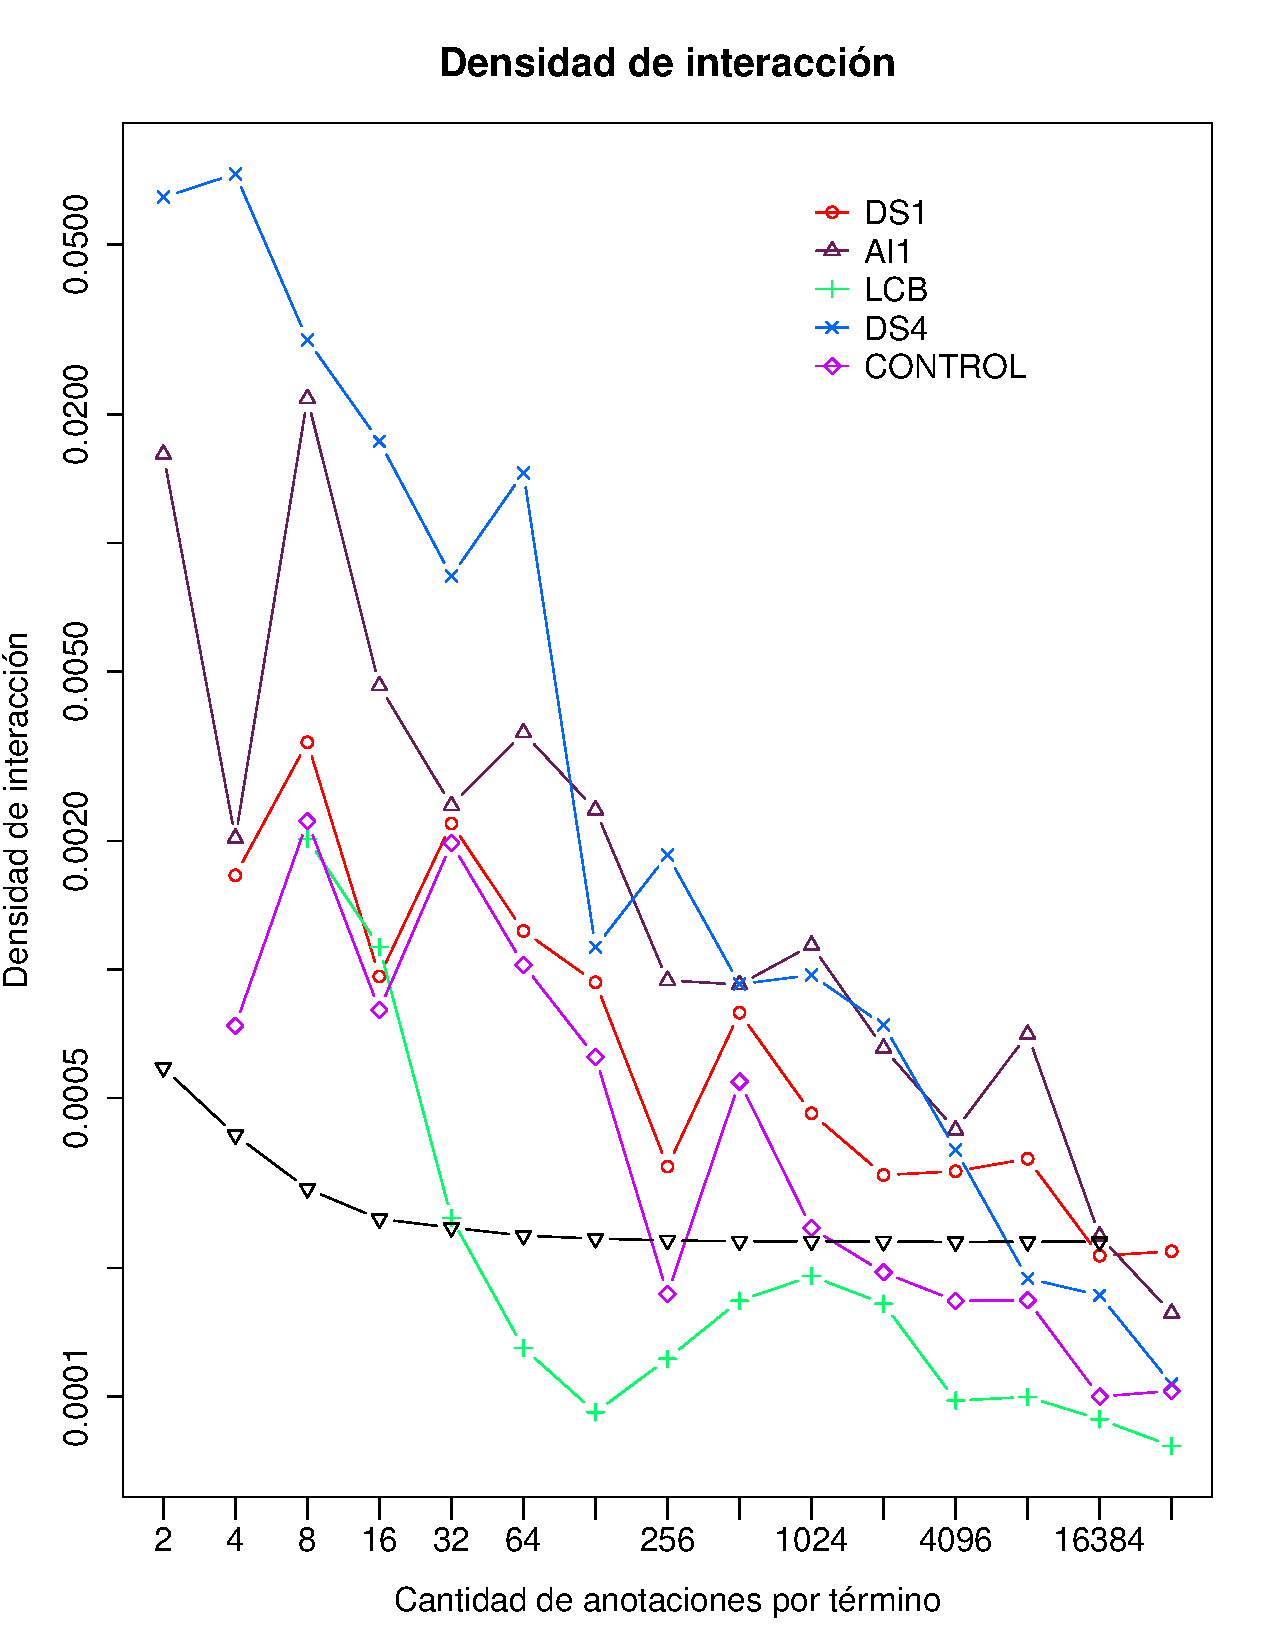
\includegraphics[width=1\textwidth]{interacting_densities_cc.pdf}
    \caption{ID para ontología CC.}
    \end{subfigure}
    \begin{subfigure}[t]{0.45\textwidth}
    \centering
    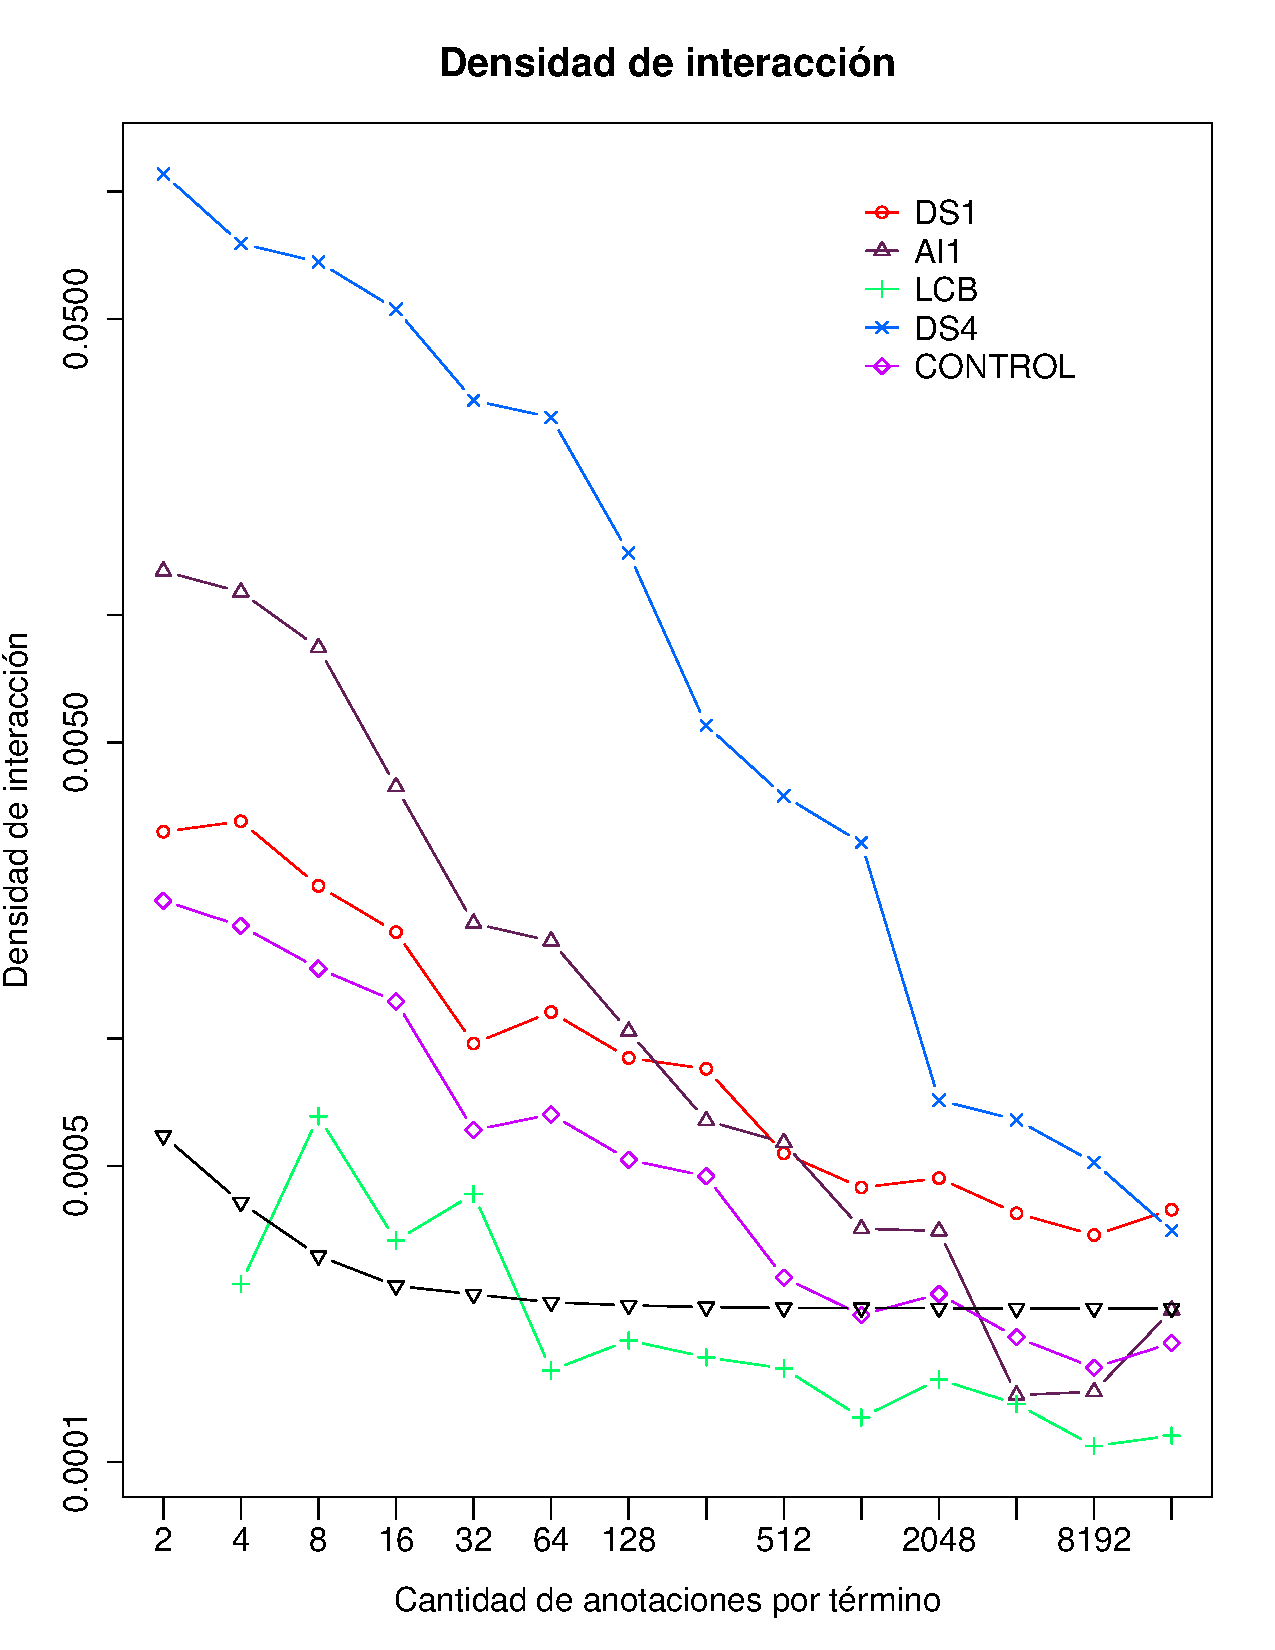
\includegraphics[width=1\textwidth]{interacting_densities_bpa.pdf}
    \caption{ID para ontología BPA.}
    \end{subfigure}
    \begin{subfigure}[t]{0.45\textwidth}
    \centering
    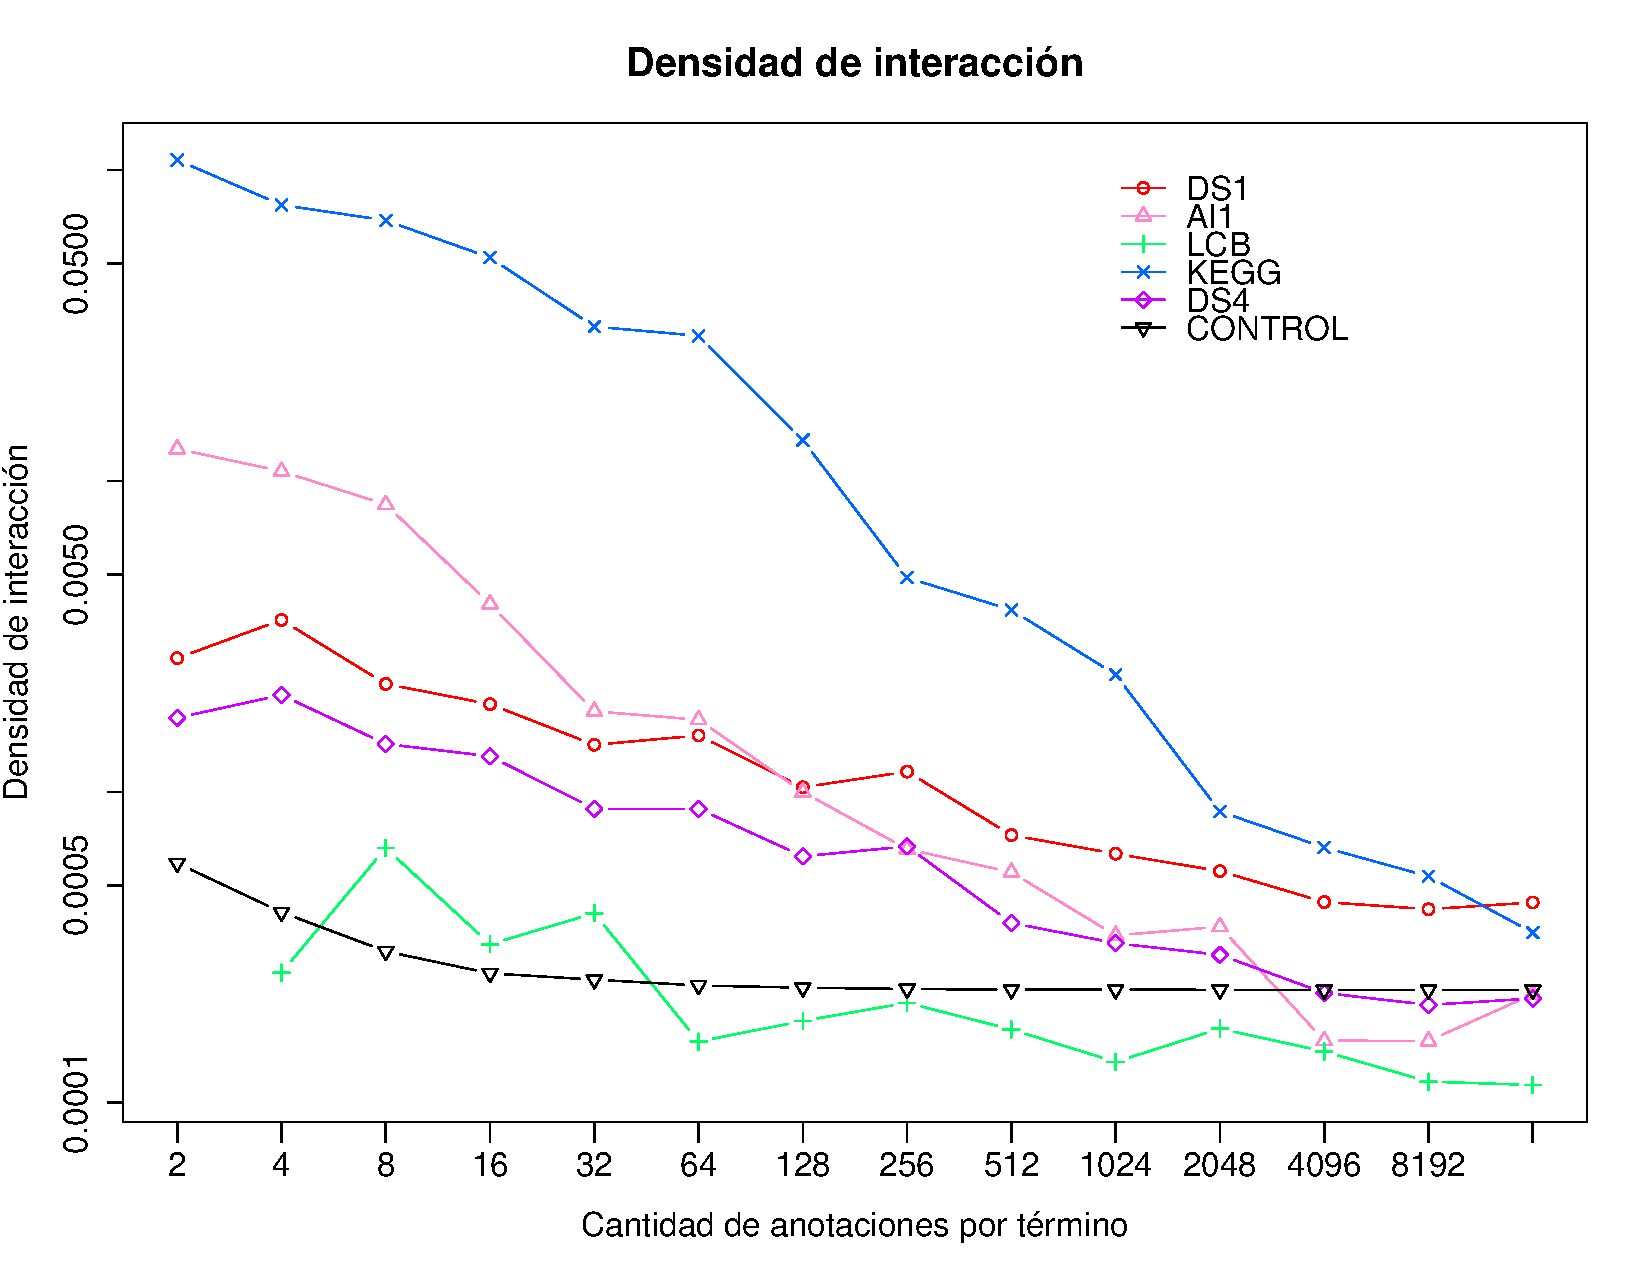
\includegraphics[width=1\textwidth]{interacting_densities_bpb.pdf}
    \caption{ID para ontología BPB.}
    \end{subfigure}    
    \caption{Índice de densidad de interacción, ID, para distintas redes de proteínas, vías metabólicas y particiones de expresión.}
    \label{interacting_densities}
\end{figure*}
Encontramos que:
\begin{enumerate}

\item En todos los casos, términos mas específicos (es decir con menos anotaciones) presentan mayor ID, de nivel notablemente superior que el control nulo, lo que sugiere que los diferentes agrupamientos hasta un tamaño relativamente grade, del orden de 100 genes, en general correlacionan con la información biológica embebida en la ontología respectiva.
\item Las estructuras detectadas en la red de interacciones metabólicas son las que presentan mayor congruencia con las ontologías. Esto es en cierta manera razonable ya que las interacciones de dicha red reflejan interacciones bioquímicas asociadas a una funcionalidad metabólica concreta.
\item Las comunidades encontradas en la red $AI1$ y luego las estructuras detectadas en el espacio transcripcional son las que siguen en cuanto a grado de congruencia general con el espacio de conocimiento de las ontologías. Esto es razonable ya que las primeras surgen de información curada de interacción de proteínas, mientras que en el caso transcripcional, la interacción entre proteínas es inferida a partir de su expresión, sin tener en cuenta posibles capas regulatorias postranscripcionales.
\item Las estructuras detectadas en el espacio transcripcional con resolución $ds1$ presentan mayor congruencia biológica, según este indicador, que aquellas obtenidas con resolución $ds4$. Esto sería un indicio acerca de cual sería la escala de granularidad apropiada para interpretar las estructuras encontradas.
\item Finalmente queremos mencionar como resultado interesante la baja coherencia encontrada para el caso de la red de interacción de proteínas $LCI$, aunque encontrar las razones de este resultado exceden los alcances de este trabajo. 
\end{enumerate}
\section{Índice de homogeneidad biológica}
El índice de homogeneidad biológica (o BHI por sus siglas en inglés) de una partición, introducido por Datta \cite{Datta2006} es un observable que cuantifica el grado en que una partición presenta grupos biológicamente homogéneos, reportando, para cada grupo, la máxima proporción de pares de genes agrupados que comparten una misma clase funcional de Ontología Génica. Consideremos dos genes $x$ e $y$ que pertenecen a un mismo grupo $D$ de una partición dada, con un total de $k$ grupos, y sean $C(x)$ y $C(y)$ los conjuntos de todas las clases funcionales que tienen anotados a los genes $x$ e $y$ respectivamente. Sea además la función indicadora $I(C(x)=C(y))$ que toma el valor $1$ si hay al menos una clase en donde ambos genes estén anotados, y $0$ en caso contrario. Entonces, el índice de homogeneidad biológica queda definido como:
\begin{equation}
	BHI = \frac{1}{k}\sum\limits_{j=1}^k\frac{1}{n_j(n_j-1)}\sum\limits_{x\neq y\in D_j}I(C(x)=C(y))
\end{equation}
con $n_j$ la cantidad de genes anotados en el grupo $D_j$.\\

\subsection{Modificaciones al Índice de homogeneidad biológica}
\label{subsec:control_nulo}
Presentaremos a continuación dos variantes del BHI que modificarán la función indicadora para hacer uso de la similaridad semántica y del contenido de información génico.\\
El índice de homogeneidad biológica con contenido de información ($BHI_{IC}$) para un grupo se define como:
\begin{equation}
	BHI_{IC} = \frac{1}{k}\sum\limits_{j=1}^k\frac{1}{n_j(n_j-1)}\sum\limits_{x\neq y\in D_j}I(C(x)=C(y))IC(C(x)\cap C(y))
\end{equation}
donde el $IC(C(x)\cap C(y))$ es el contenido de información del término más informativo en el que ambos genes se encuentran anotados.\\
Este índice permite pesar la homogeneidad biológica de un grupo utilizando la especificidad de los conceptos en coincidencia.\\
Por otro lado, el índice de homogeneidad biológica Resnik para un grupo, $BHI_{Resnik}$ queda definido como:
\begin{equation}
	BHI_{Resnik} = \frac{1}{k}\sum\limits_{j=1}^k\frac{1}{n_j(n_j-1)}\sum\limits_{x\neq y\in D_j}Sim_{rcmax}(C(x), C(y))
\end{equation}
donde $Sim_{rcmax}(C(x), C(y))$ es la similaridad biológica entre los genes x e y.\\
Este índice pesa la homogeneidad biológica de un grupo por la similaridad semántica de los genes que lo componen.\\
Finalmente, el índice de homogeneidad biológica estandarizado para un grupo, zBHI, utiliza como referencia los valores obtenidos en situaciones triviales, sin estructura y se define como:
\begin{equation}
	zBHI = \frac{BHI-<BHI_r>}{s(BHI_r)}
\end{equation}
donde $<BHI_r>$ es el valor medio del conjunto de valores del BHI del grupo para un control nulo de 1000 reasignaciones de las etiquetas de la partición y $s(BHI_r)$ es la desviación estandar de la muestra para el mismo conjunto.\\
Se realizaron además dos tipos de controles nulos.\\
El primero, un control nulo que llamaremos ``control nulo 1'', se realizó considerando agrupamientos aleatorios (de tamaños variables) a partir de un conjunto de los aproximadamente 6000 genes que pasaron el filtrado en al menos un tratamiento analizado. Para cada tamaño de agrupamiento analizado (entre 2 y 500 genes), se realizaron 1000 grupos aleatorios y se calculó su BHI. Se encontró que el valor medio de los ensambles se mantenía aproximadamente constante, mientras que existía una dependencia de la desviación estandar con el tamaño de los grupos. Se realizaron dos ajustes por funciones de ley de potencias, para tamaños entre 1 y 50 y de 51 en adelante. Las funciones halladas permiten rápidamente obtener el BHI aleatorio medio para una partición de cualquier tamaño y su desviación estandar.\\
El segundo, que llamaremos ``control nulo 2'', consistió en realizar 1000 reasignaciones aleatorias de las etiquetas de cada partición y calcular el BHI de cada grupo de la misma. Encontramos que la media de BHI calculada de esta manera coincidía con la del control nulo anterior, pero no así su desviación estándar. Concluimos que la diferencia fundamental se basa en que en el segundo caso, en la reasignación de etiquetas, se mantiene siempre la estructura de tamaños de la partición, mientras que en el primer caso, cada grupo fue tomado por separado.\\
Para caracterizar el comportamiento de cada uno de estos índices se midieron los mismos para cada tratamiento y se calculó su correlación de a pares de índices. La figura \ref{fig:correlacion_de_a_pares_bhi} muestra las distribuciones y correlaciones de a pares para estos índices en el tratamiento ``Frío''. Se encuentra que los índices modificados tienen una alta correlación entre ellos y con BHI. Esto pareceria indicar que no aportan más información que la que se obtiene a través del índice original. Por ser el más sencillo de calcular, es el que utilizaremos como criterio de validación externa de la calidad de una partición.
\begin{sidewaysfigure}
    \centering
    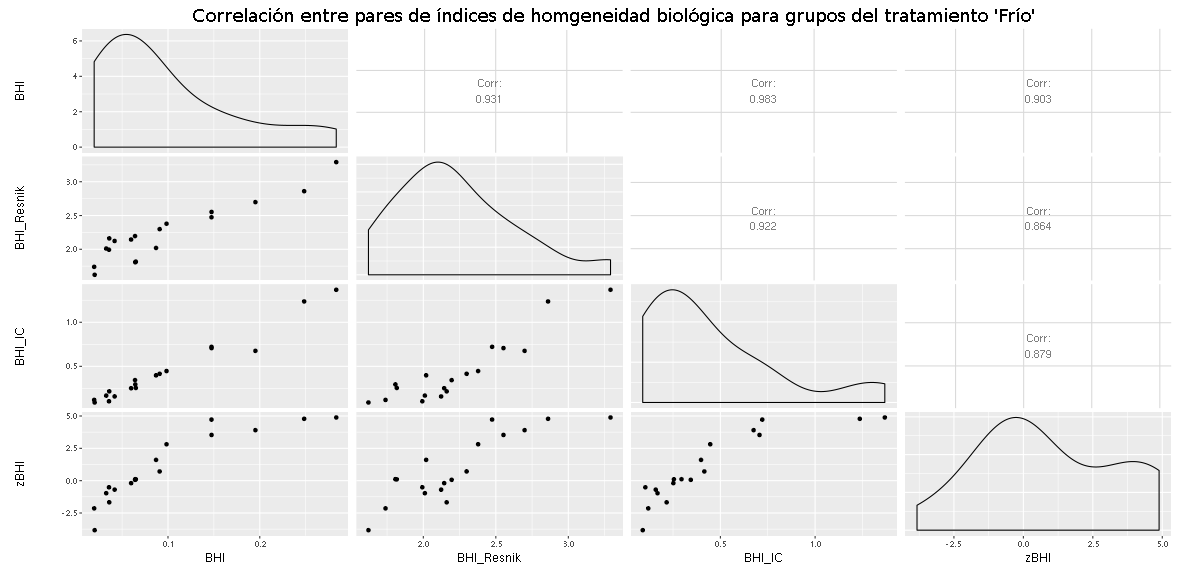
\includegraphics[width=0.9\textheight]{correlacion_de_a_pares_bhi}
    \caption{Correlación de a pares para los distintos índices de homogeneidad biológica presentados para cada uno de los grupos del tratamiento 'Frío' obtenidos con $ds=1$. Se observa que todos los índices tienen una alta correlación entre si.}
    \label{fig:correlacion_de_a_pares_bhi}
\end{sidewaysfigure}


\section{Congruencia biológica de las particiones transcripcionales}
Los valores de BHI calculados para cada uno de los grupos del tratamiento ``frío'' en las particiones k-means (puntos rojos), $ds1$ (triángulos verdes) y $ds4$ (cuadrados azules) se presentan en las figuras \ref{fig:bhi_km_ds1_ds4_control1}, con control nulo 1 y \ref{fig:bhi_km_ds1_ds4_control2} con control nulo 2. Los grupos fueron ordenados según su masa de forma creciente.\\
Se observa que de los dos grupos de kmeans, solo uno presenta un BHI superior a una desviación estandar para el control nulo 1 y del tercer cuartil para el control nulo 2, mientras que para $ds1$, el 45\% de los grupos superan una desviación estandar para control nulo 1 y el 30\% de los grupos superan el tercer cuartil para el control nulo 2.
\begin{figure*}[t!]
    \centering
    \begin{subfigure}[t]{0.8\textwidth}
    \centering
    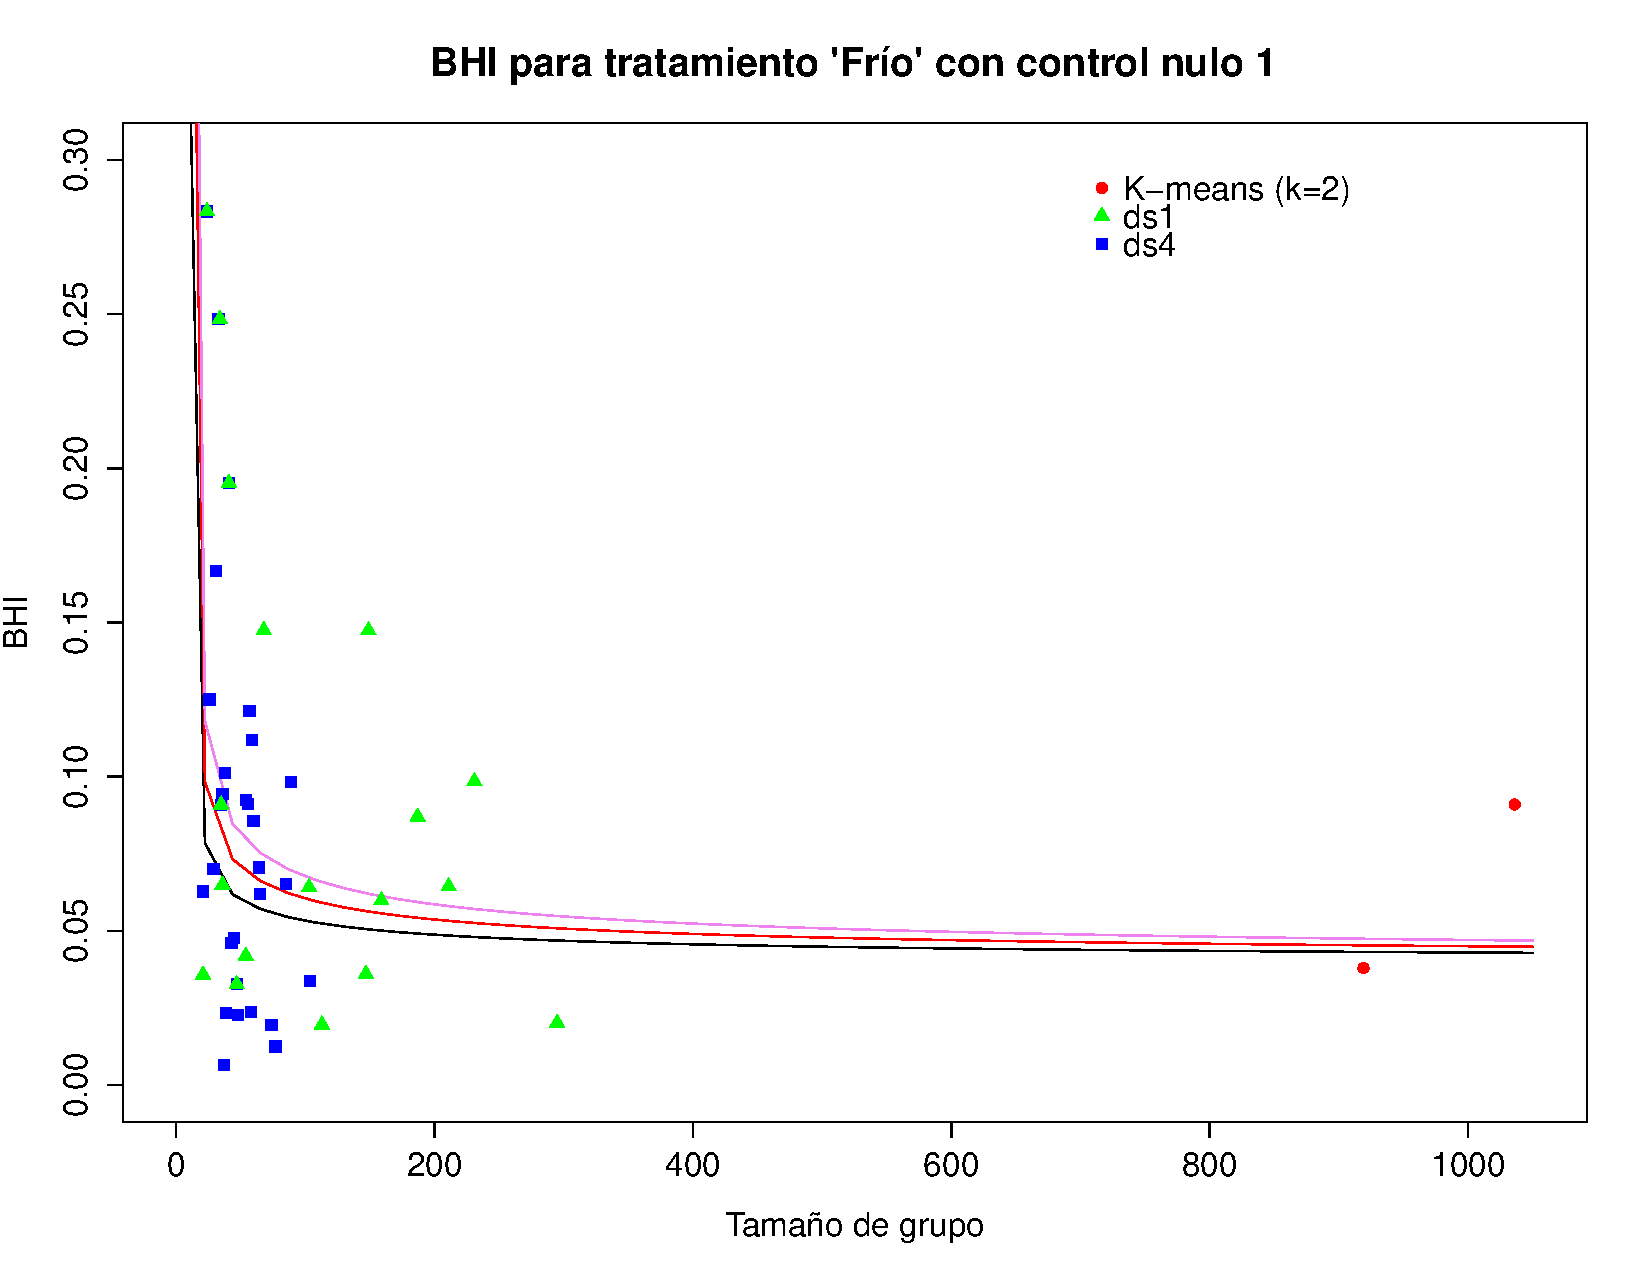
\includegraphics[width=1\textwidth]{bhi_km_ds1_ds4_control1.pdf}
    \caption{BHI para cada uno de los grupos del tratamiento 'Frío' obtenidos con kmeans, $ds1$ y $ds4$ y control nulo 1. En rojo, el valor medio del BHI, en violeta una desviación estándar por sobre el valor medio y en negro una desviación estandar por debajo del mismo.}
    \label{fig:bhi_km_ds1_ds4_control1}
    \end{subfigure}
    \begin{subfigure}[t]{0.8\textwidth}
    \centering
    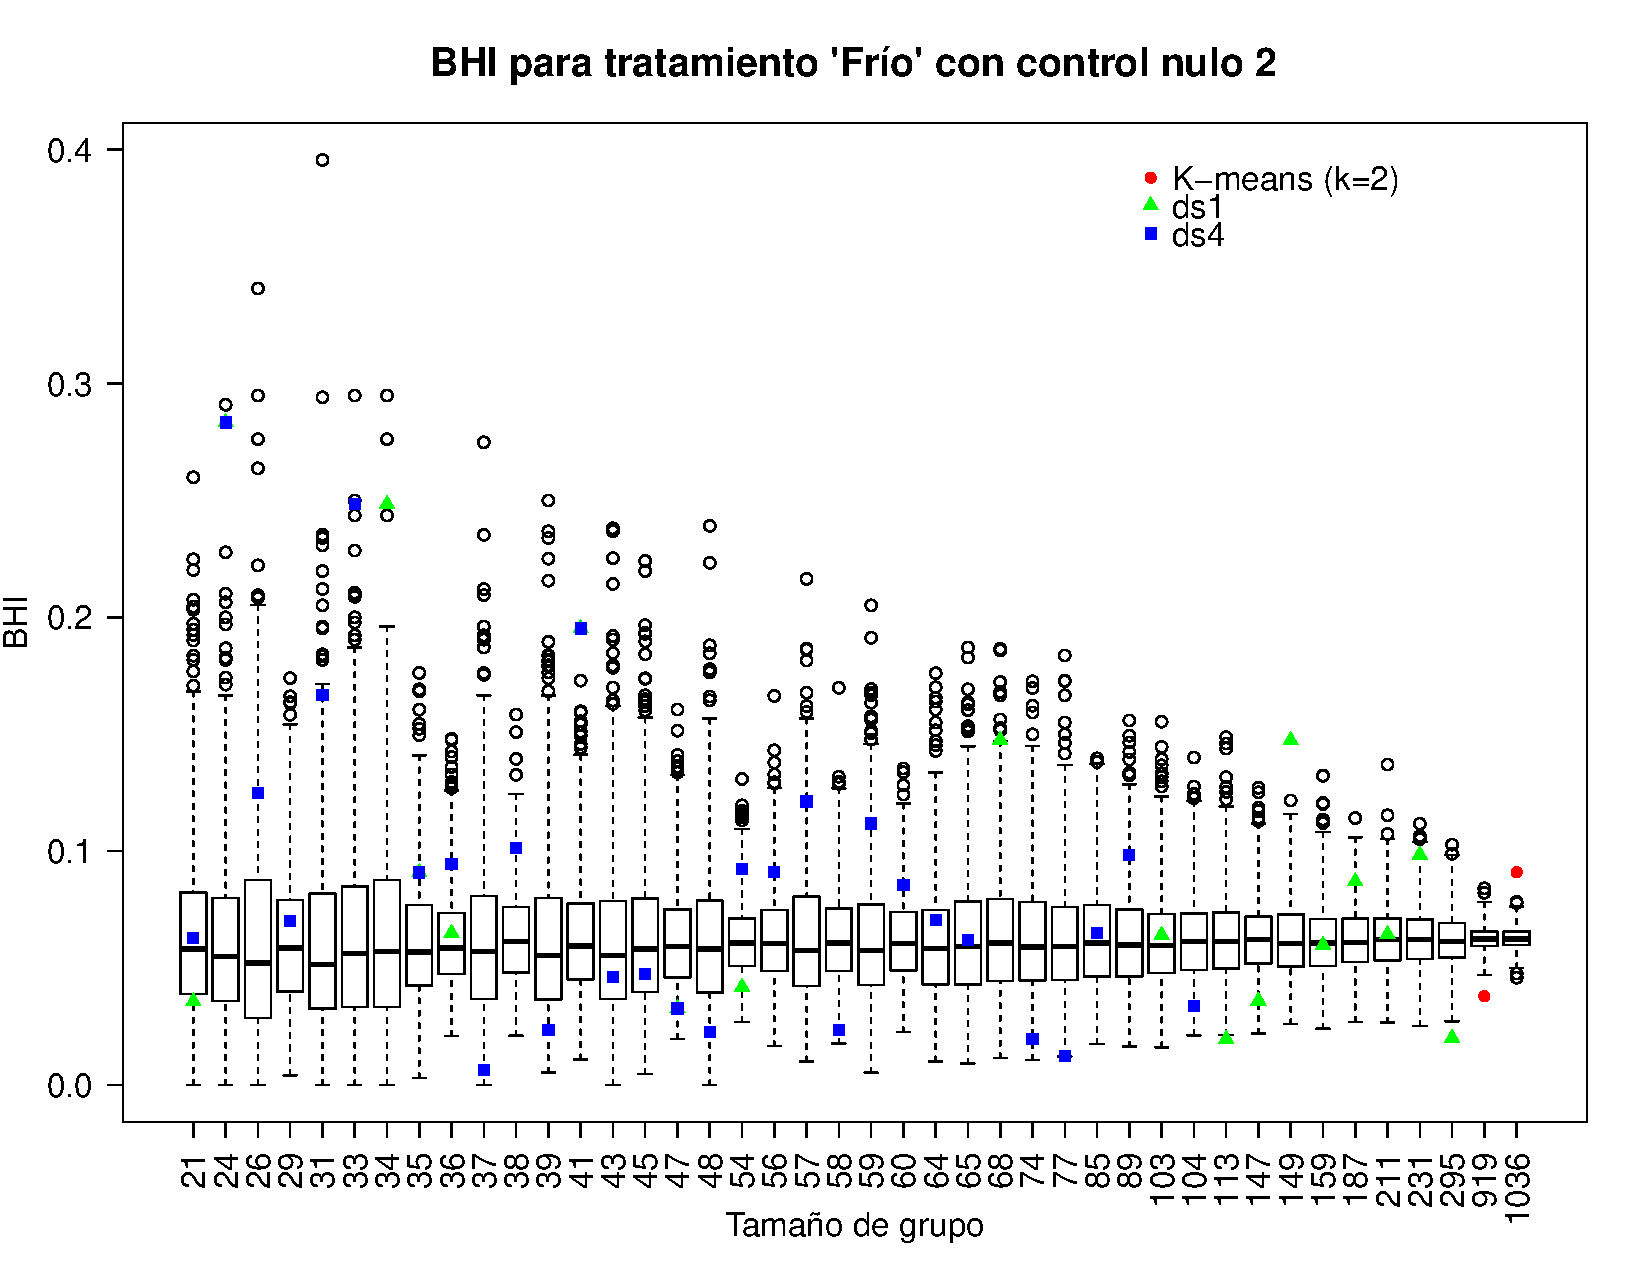
\includegraphics[width=1\textwidth]{bhi_km_ds1_ds4_control2.pdf}
    \caption{BHI para cada uno de los grupos del tratamiento 'Frío' obtenidos con kmeans, $ds1$ y $ds4$, y control nulo 2.}
    \label{fig:bhi_km_ds1_ds4_control2}
    \end{subfigure}
    \caption{Índice de Homogeneidad Biológica, BHI, para cada uno de los grupos del tratamiento 'Frío' obtenidos con kmeans, $ds1$ y $ds4$ y controles nulos.}
\end{figure*}

Finalmente, para la partición $ds4$, aproximadamente el 40\% de los grupos presenta un BHI por sobre una desviación estandar para el control nulo 1 y un 50\% presenta un BHI por sobre el tercer cuartil del control nulo 2.\\ 
Esta baja calidad en el índice BHI de las particiones se encontró de forma similar a lo largo de todos los tratamientos. Esto sugiere que si bien el aumentar la granularidad de la partición con el método corte de árbol dinámico resulta en un aumento de la consistencia biológica global de las estructuras observadas, esto no implica que las resoluciones utilizadas sean las óptimas, ya que por lo general el BHI no es superior al del control nulo.\\
A pesar de que en el análisis de estructura de los grupos obtenidos por medio de los métodos k-means, $ds1$ y $ds4$ encontramos que todos los métodos producen particiones altamente coherentes, el análisis de BHI indica que las particiones halladas no pueden ser fácilmente interpretadas a la luz del conocimiento biológico almacenado en GO.\\
En el próximo capítulo buscaremos cuantificar la coherencia entre los espacios de expresión genética y de conocimiento biológico desde una perspectiva diferente: desde la métrica en lugar de desde las agrupaciones.
